\selectlanguage{italian}%

\section{Soluzione}


\subsection{Schematici}

\begin{figure}[H]
	\centering
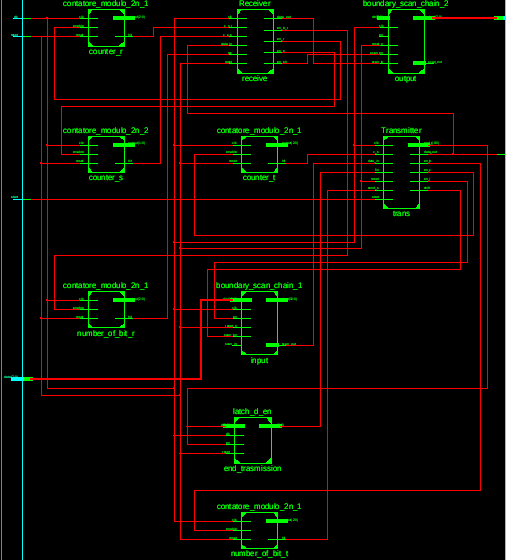
\includegraphics[scale=0.65]{esercizio15/images/UART.png}
	\caption{UART}
\end{figure}

Si � realizzata una versione di UART secondo lo schema PO/PC, i componenti
principali solo le due macchine a stati finiti:
\begin{itemize}
\item il trasmitter che consiste di cinque stati: 
\begin{itemize}
\item idle, rimane in attesa fino a che non si decide di avviare una trasmissione;
\item send\_start invia il segnale di start; 
\item wait\_for\_next attende fino a che il contatore counter\_t non genera
un segnale di counter hit, per far s� prima che venga inviata la successiva
informazione, quella attuale venga sorretta per sedici colpi di clock; 
\item send che abilita lo shifting della scan chain con il dato ingresso
per invare il successivo bit;
\item send\_stop che invia il bit di stop, si abilita questo stato quando
il numero di bit trasmetti � pari ad otto (il conteggio � fissato
da un contatore).
\end{itemize}
\item Il ricevitore invece � composto solo da quattro stati: 
\begin{itemize}
\item idle, si permane in questo stato fino a quando la linea dei dati in
ingresso � alta; 
\item sfasamento fa in modo di posizionare l' evento di lettura del dato
a met� del tempo per il quale � sorretto il dato, cos� da essere sicuri
di leggere correttamente il bit;
\item wait\_for\_next dove si attende per leggere il successivo bit; 
\item receive dopo si effettua la lettura del bit in ingresso.
\end{itemize}
\end{itemize}
%
Il ricevitore ha diversi contatori, uno che tiene in conto del numero
di bit letti affinch� dopo aver letto l' ottavo si ritorna in idle,
un altro che conta il numero di cicli di clock per lo sfasamento ed
infine uno che conta il numero di colpi di clock da attendere prima
di leggere il successivo dato. 

I dati in input ed in output sono sorretti da due scan chain come
quelle utilizzate in Booth \ref{Booth}, quella dell' input � pi�
grande di tre bit perch� vi � un primo bit alto per indicare che non
vi � trasmissione di dati fino a che non vi � un invio di dati, il
secondo � il bit di start ed il terzo messo in coda ai dati � quello
di stop.

Premettendo che la soluzione di Digilent effettua vari controlli sulla
trasmissione qui non effettuati, la riteniamo di non facile comprensione,
scrivere in un unico file VHDL sia il ricevitore, trasmettitore, i
contatori e tutti gli altri componenti a supporto non permette di
rendere chiara la lettura, non � lampante quali parti siano a supporto
del ricevitore e quali del ricevitore, non permettendo cos� una modifica
veloce nel caso in cui volessimo attendere ad esempio trentadue cicli
di clock prima di inviare ricevere un altro dato o estrapolare uno
solo dei due componenti e riutilizzarlo (pensiamo al caso in cui dobbiamo
solo inviare i dati e non riceverli), invece nella nostra soluzione
possiamo estrapolare una delle due macchine a stati finiti all' occorrenza
e nell' unico file in cui sono riacchiusi i componenti a corredo capire
quali ci occorrono ed riutilizzarli, oppure in base ai segnali in
ingresso alle due macchine sequenziali capire quali segnali ci possano
occorrere, altro punto a sfavore � la realizzazione di diversi process
per fare andare la macchina ad una frequenza voluta per trasmettere/ricevere
ad un determinato baud rate, soluzione migliore consisterebbe di utilizzare
un DCM e cambiare la frequenza in base alla necessit�.

\subsection{Codice}

\href{run:progetti/UART/UART.xise}{UART ISE}

\selectlanguage{italian}%

